\documentclass[9pt,twocolumn,twoside]{../../styles/osajnl}
\usepackage{fancyvrb}
\journal{i524} 

\title{Head Count Detection Using Apache Mesos}

\author[1,*]{Anurag Kumar Jain}
\author[1,*]{Pratik Sushil Jain}
\author[1,*]{Ronak Parekh}

\affil[1]{School of Informatics and Computing, Bloomington, IN 47408, U.S.A.}

\affil[*]{Corresponding authors: jainanur@iu.edu, jainps@iu.edu, parekhr@iu.edu}

\dates{Project P011, \today}

\ociscodes{Cloud, I524, Apache Mesos, OpenCV, Face detection, Mesospehere, Ansible, Big Data, Zookeeper, Marathon, Haar Cascade}

% replace this with your url in github/gitlab
\doi{\url{https://github.com/cloudmesh/sp17-i524/blob/master/project/S17-IR-P011/report.pdf}}

\begin{abstract}
Apache Mesos can be used for scaling of applications and providing
highly available clusters. It provides the functionality to use
resources from multiple agents and execute the application using the
offered resources. Deployment of a custom face detection application
is done using Ansible on Apache Mesos and analysis of the deployments
are benchmarked. The face detection application was created using
OpenCV. Ansible playbooks are used to deploy Apache Mesos on virtual
machines created on chameleon cloud. For benchmarks, deployment of
Mesos on different systems and different sizes of virtual machines
were carried out.
\newline
\end{abstract}

\setboolean{displaycopyright}{true}

\begin{document}

\maketitle

\section{Introduction}
There are a number of applications which require the counting of
people in an image. The application for detecting headcount in an
image can be in the field of attendance management and tagging images
on social media. The purpose of this project is to deploy a head count
detection framework on Apache Mesos to enable distributed processing
of image data over the cloud. Apache Mesos is built using the same
principles as the Linux kernel but at a different level of
abstraction. It runs on every machine and provides applications with
API's for resource management and scheduling across different cloud
infrastructures \cite{www-mesos}. Ansible is used to automate the
deployment of the head count detection application on Apache Mesos
which will be deployed on Chameleon cloud. The VGG face detection
dataset is used for benchmarking the performance of Mesos on different
versions of the Linux Operating System. The head count detection is
restricted to detection of the number of frontal faces in an image
\cite{www-face-detection-wikipedia}. This is due to the field of face
detection and image processing being vast and thus the head count
detection is restricted to detecting faces based on simple
criteria. The performance benefits of Apache Mesos in terms of high
availability, scalability and fault tolerance are leveraged by
deploying the application on a virtual machine which offers its
computing resources to Mesos for fast computation.

\section{Why Mesos?}
Mesos can be used to implement a decentralized scheduling approach. In
this approach, each framework decides which offers to accept or
reject. There are many incentives that are provided by any
decentralized system. The incentives provided by Apache Mesos system
includes short tasks, no minimum allocation, scale down and not
accepting unknown resources \cite{www-mesos-paper}.

\section{What is Mesos?}
Mesos is built using the same principles as the Linux kernel. However,
it is at a different level of abstraction. The Mesos kernel runs on
every machine and provides applications such as Hadoop, Spark, Kafka,
Elastic Search with API's for resource management and scheduling
across entire cloud environments and data center \cite{www-mesos-paper}.

\subsection{Design Philosophy}
Mesos aims to provide a resilient core to enable various frameworks
for efficient cluster sharing. As cluster frameworks are rapidly
evolving and highly diverse, this overriding design philosophy
focussing on defining a minimal interface enabling efficient
resource sharing across frameworks and otherwise push control of task
scheduling and execution to the frameworks. Pushing control to the
frameworks has two benefits. It allows frameworks to implement diverse
approaches to various problems in the cluster and to evolve these
solutions independently. This also keeps Mesos simple and minimizes
the rate of change required, which makes it easier to keep Mesos
scalable and robust. Higher level libraries implementing common
functionality are built on top of Mesos even though Mesos provides a
low-level interface. Including the functionality in libraries rather
than in Mesos allows it to remain small and flexible and lets the
libraries evolve independently.

\subsection{Architecture}

\begin{figure}[htbp]
\centering
\fbox{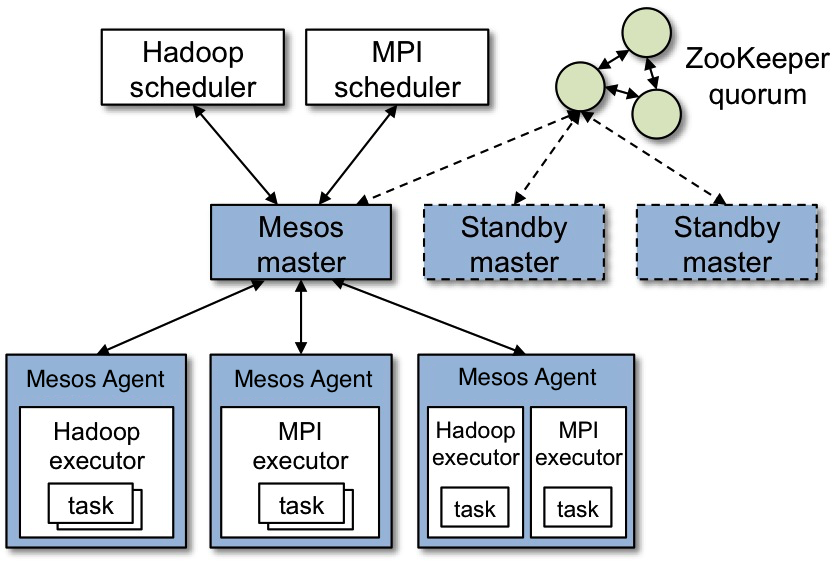
\includegraphics[width=\linewidth]{images/mesos_arch_1}}
\caption{Mesos architecture \cite{www-mesos-arch}.}
\label{fig:false-color}
\end{figure}

Mesos consists of a master daemon through which an agent running on
each cluster node is managed. It also consists of a Mesos Framework
that runs tasks on these agents.  The master enables the fine-grained
sharing of resources including CPU and RAM across all the frameworks
by making resource offers. Each resource offer contains a list of
<agent ID, resource1:amount1, resource2: amount2,...>
\cite{www-mesos-arch}. The master decides how many resources to offer
to each framework based on an organizational policy such as strict
priority or fair sharing. A diverse set of policies is supported by
employing a modular architecture that makes it easy to add new
allocation modules via a plug-in mechanism \cite{www-mesos}.

A framework running on top of Mesos consists of two components: an
executor process that can be launched on agent nodes to run framework
tasks and a scheduler that registers with the master to the resource
offered. While the master determines how many resources are offered to
each framework, the framework scheduler selects which of the offered
resources to use. When a framework accepts offered resources, the
description is passed to Mesos \cite{www-mesos-arch}.

The sequence of events in the figure are as follows:
\begin{enumerate}
\item Agent 1 reports to the master that it has 4 CPU's and 4GB of
  memory free.  An allocation policy module is invoked by the master
  which tells it that framework 1 should be offered all available
  resources \cite{www-mesos-arch}.
\item The master sends a resource offer to framework 1 which includes
  details of which resources are available on agent 1.
\item A reply is sent back to the master by the frameworks scheduler
  with information regarding two tasks to run on the agent, using
  <2CPU's, 1 GB RAM> for the first task, <1CPU and 2 GB RAM> for the
  second task \cite{www-mesos-arch}.
\item Finally the master sends the task to the agent which allocates
  appropriate resources to the frameworks executor which in turn
  launches the two tasks. The allocation module may now offer the
  unallocated resources to framework 2 \cite{www-mesos-arch}.
\end{enumerate}

\begin{figure}[htbp]
\centering
\fbox{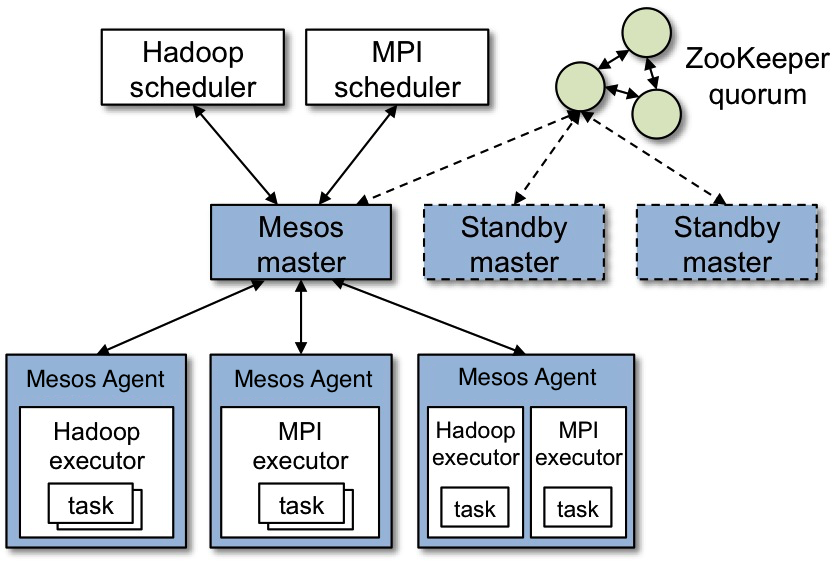
\includegraphics[width=\linewidth]{images/mesos_arch_1}}
\caption{Example Flow \cite{www-mesos-arch}.}
\label{fig:false-color}
\end{figure}

The resource offer process repeats when new resources become free or
when tasks are finished.

\section{Mesos Framework}
A Mesos Framework is used to manage tasks. A Mesos framework is highly
available only if it continues to manage tasks correctly in the
presence of a variety of failure scenarios. There are failure
conditions which the framework should consider. The conditions are as
follows:

\begin{itemize}
\item A framework scheduler which is connected to a Mesos master might
  fail. It may be due to crashing or losing network connectivity. If
  the master has been configured to use the high availability mode,
  this will promote a replica of another Mesos master to become the
  new leader. In this case, the scheduler re-registers with the new
  master and ensure the task state is consistent
  \cite{www-mesos-frmwrk}.
\item A host may fail where a framework scheduler is running. While
  creating the framework, the framework authors should ensure that
  multiple copies of the scheduler run on different nodes and a backup
  copy is promoted to become the new leader where a previous leader
  fails. This is done to ensure that the framework remains available
  and can continue to run new tasks \cite{www-mesos-frmwrk}.
\item The host might fail on which a task is running. The node might
  not have failed but the Mesos agent on the node might be unable to
  communicate with the Mesos master due to a network partition
  \cite{www-mesos-frmwrk}.
\end{itemize}

\subsection{Internal Working of Framework}
When the agents are connected to the Mesos master, they offer
resources to the Mesos master in terms of CPU's, RAM and disk
space. These resources are available for the master to use till the
agents are in the active state. There can be multiple states for the
Mesos agents such as Active state, Deactivated state and Unreachable
state. When an agent is successfully able to connect to the master, it
is in the active state. When an agent is not able to advertise its IP
address to the master, the agent state is changed to deactivated. If
there are network outages and the agent is unable to reach the master,
it goes in the unreachable state. The master is able to use the
resources offered by the agent only if the agent is in the active
state. When the face detection framework is started on Mesos master,
the master searches for any available resource offers from the active
agents. It breaks the execution of the framework into multiple tasks
and uses the resource offers to execute the task. The task runs on
multiple CPU's if available, and after completion of each task a
status update is sent to the Mesos master. Each individual task is
assigned a unique task id. If an agent doesn't update the status of
the task due to network outage or failure of the agent, the Mesos
master persists the task id and it assigns the task id to a new agent
which has resources available and the task is resumed. The framework
state changes to active when the tasks of the framework are running
and changes to completed when the execution of the framework is
finished.

\subsection{Highly Available Frameworks}
Mesos provides unreliable messaging between components by default:
Messages are delivered at most once by default. Framework authors
should take into consideration that the messages they sent might not
be received and should be prepared to take corrective action. Timeouts
are used to detect whether a message is lost. There are situations
where the framework attempts to launch a task but the message does not
reach the Mesos master \cite{www-mesos-frmwrk}. To address such issues
a framework scheduler should set a timeout after attempting to launch
a new task. The scheduler should take corrective action if the
scheduler does not receive a status update and thereby launching a new
copy of the task \cite{www-mesos-arch}.

In general, distributed systems cannot distinguish between 'lost'
messages and messages that are delayed. There might be a case where
the scheduler might see a status update for the attempt of the first
task launch immediately after its timeout has fired but it has already
begun to take corrective action.  Mesos provides ordered message
delivery between any pair of processes. If a framework sends a message
M1 and M2 to the master, then the master might not receive any
messages, or it may receive only M1 or, only M2 or, M1 followed by
M2. But it will never receive messages in the order M2 followed by M1
\cite{www-mesos-frmwrk}.  Mesos also provides reliable delivery of the
task status updates.  The agent persists task status updates to disk
and then forwards them to the master.  The master sends status updates
to the appropriate framework scheduler.  When a scheduler acknowledges
a status update, the master forwards the acknowledgment back to the
agent, which allows the stored status update to be garbage
collected. If the agent does not receive an acknowledgment for a task
status update within a specific amount of time, it will repeatedly
resend the status update to the master, which will again forward the
update to the scheduler. Hence, task status updates will be delivered
``at least once'', assuming that the agent and the scheduler both
remain available \cite{www-mesos-frmwrk}.

The information about the active tasks and registered frameworks is
stored by the Mesos master in memory.  Persistent storage is not used
and it does not ensure that the information is preserved even after
the master is failed.  This feature helps the Mesos master to scale to
large clusters with many tasks and frameworks \cite{www-mesos-frmwrk}.
If all the Mesos masters are unavailable or crashed, the cluster
should continue to operate.  The existing Mesos agents and user tasks
should continue running but new tasks cannot be scheduled and
frameworks will not receive resource offers or status updates about
previously launched tasks. Mesos does not dictate how frameworks
should be implemented and does not try to assume responsibility for
how frameworks should deal with failures \cite{www-mesos-frmwrk}.

\subsection{Designing Highly Available Frameworks}
The patterns followed for designing highly available networks are as follows:
\begin{itemize}
\item Frameworks run multiple scheduler instances to tolerate
  scheduler failures. Only one of the scheduler instances is the
  leader at any particular given point in time. This instance is
  connected to the Mesos master, it receives resource offers and task
  status updates and launches new tasks. The other available
  scheduler replicas are followers. They are used only when the leader
  fails and in that case one of the followers is chosen to become the
  new leader via polling \cite{www-mesos-frmwrk}.
\item The election of a new leader is done via a mechanism and
  schedulers need that mechanism when the scheduler has failed. This
  mechanism is typically provided using a coordination service. This
  coordination service can be Apache ZooKeeper \cite{www-mesos-frmwrk}.
 \item After election is conducted and a new leading scheduler is
   elected, the new leader should reconnect to the Mesos master. When
   the master is registered, the framework should set the id field in
   its FrameworkInfo to the ID that was assigned to the failed
   scheduler instance. This ensures that a new session is not started
   by the master and the master recognizes the connection. Thus, it
   will continue the session used by the failed scheduler instance.
 \item After connecting to the Mesos master, the newly elected leading
   scheduler should maintain the consistency of its local state with
   the current state of the cluster. If the previous leading scheduler
   attempted to launch a new task and then failed immediately, the
   task might have launched successfully and the newly elected leader
   will start to receive updates regarding it
   \cite{www-mesos-frmwrk}. Frameworks typically use a consistent
   distributed data store to record information about active and
   pending tasks. The coordination service that is used to elect the
   master can be used for this purpose. Mesos replicated logs can also
   be used to achieve this. The data store is used to record the
   actions that the scheduler intends to take, before it takes
   them. If a scheduler intends to launch a task, it first writes this
   intent to its data store. It then sends a launch task message to
   the Mesos master. This helps in cases when the instance of the
   scheduler fails and a new scheduler is promoted to become the
   leader, the newly elected leader then consults the data store to
   find all the possible tasks that might be running on the cluster.

   The approach is called as write-ahead logging pattern. The key
   aspects of this approach can be summarized as one when the
   scheduler must persist its intent before launching task. If the
   task is launched and then the scheduler fails before it can write
   to the data store, the new scheduler instance is unaware of the
   new task. In this case, the new scheduler instance will begin
   receiving the task status updates for a task it has no
   knowledge of. Another aspect is that the scheduler should ensure that
   its intent has been durably recorded in the data store before it
   continues to launch the task \cite{www-mesos-frmwrk}.
\end{itemize}

\section{Life Cycle of a Task}
A Mesos task transitions through a sequence of states. The agent is
the actual source from which the state of a task can be
determined. The agent on which the task is running provides
information regarding the actual state of the task. The framework
scheduler learns about the current state of the task by communicating
with the Mesos master \cite{www-mesos-arch}. It does learn by
listening for task status updates and performing task state
reconciliation.  The task states are represented by the frameworks
using a state machine. It can have one initial state and possibly
several terminal states \cite{www-mesos-frmwrk}.

TASK\_STAGING state is the first state of the task. The task begins in
the TASK\_STAGING state and is in this state when the framework sends
the request to the master. The master receives the request to launch
the task but the task has not yet started to run
\cite{www-mesos-frmwrk}.

TASK\_STARTING state is intended to be used by executor which are
custom implemented. This state can be used to describe that a custom
executor is aware of the task and might have started fetching its
dependencies but it hasn't yet started \cite{www-mesos-frmwrk}.

TASK\_RUNNING is the state when a task transitions to after it has
begun running successfully. The framework should perform
reconciliation when it attempts to launch a task but does not receive
a status update within a particular timeout interval. For unknown
tasks, the master will reply with the TASK\_LOST status. The framework
uses this to distinguish between the tasks that are slow to launch and
the tasks that the master is unaware about \cite{www-mesos-frmwrk}.

TASK\_KILLING state is an optional state which is intended to indicate
that the request has been received by the executor but the
corresponding task has not yet been killed. This might be useful for
tasks to be killed smoothly.  Executors should not generate this state
unless the framework has the TASK\_KILLING\_STATE capability
\cite{www-mesos-frmwrk}.

There are several terminal states such as TASK\_FINISHED which depicts
when a task is completed successfully, TASK\_FAILED indicates that the
task is aborted with an error, TASK\_KILLED indicates that a task was
killed by the executor, TASK\_LOST depicts that the task was running
on an agent that has lost contact with its master and TASK\_ERROR
indicates that a task is launched but its attempt to launch the task
has failed because of an error in the task specification
\cite{www-mesos-frmwrk}.

\section{Comparison of Mesos, Docker and Kubernetes}
Mesos, Kubernetes and Docker fall into DevOps infrastructure
management tools known as Container Orchestration Engines(COEs)
\cite{mesos-cmp}. An abstraction layer of protocols are provided by
COEs between a pool of resources and the containers of application
that run on these resources. COEs also solve the problem of taking
multiple discrete resources in the cloud and combine them into a
single pool. This pool can be used to deploy a variety of
applications. These tools provide a set of features such as Container
scheduling, High Availability, Health checks, Service discovery and
Load balancing. Container scheduling comprises of performing functions
which start and stop containers, distributing containers amongst
pooled resources, failure recovery of containers, rebalancing
containers from hosts that are failed to hosts that are healthy and
scaling of applications \cite{mesos-cmp}. High availability of
application and container is provided by these tools. The health
checks are used to determine the container and application health
while service discovery is used to determine the services which are
located on a network \cite{mesos-cmp}.

\subsection{Kubernetes Container Orchestration Capailities}
Kubernetes project originated to resolve the issue of running
containers at a massive scale. Kubernetes uses YAML-based deployment
model. It is used to manage the scheduling the containers on host
machines. It also includes features such as built-in auto-scaling,
secrets management, load balancing and volume management. It requires
less third party software than Mesos and Swarm. It consists of a
concept of pods which are groups of containers that are scheduled
together to form a service. It doesn't support single node master
installations with highly available clusters. The learning curve of
Kubernetes is steeper than Swarm.

\subsection{Swarm Container Orchestration Capabilities}
Docker Swarm is a native Docker Container Orchestration Engine. Swarm
is tightly integrated with the Docker API which makes it extremely
suitable for its use with Docker. Swarm uses the same primitives as
applicable to single host docker cluster. It simplifies managing
container infrastructure as there is no need to configure a different
orchestration engine. Swarm also uses a YAML-based deployment model
using Docker Compose. Its main features includes auto-healing of
clusters, overlay networks with DNS, and usage of multiple masters for
high availability. Swarm does not support native auto-scaling as well
as external load balancing. Swarm includes the capability of ingress
load balancing but it requires a third party load balancer for
external load balancing.

\subsection{Mesos Container Orchestration Capabilities}
Apache Mesos takes a more distributed approach to managing datacenter
and cloud resources. Mesos uses Zookeeper to manage multiple masters
and form a high-availability cluster. Other container management
frameworks can be run on top of Mesos including Kubernetes, Apache
Aurora, Chronos, and Mesosphere Marathon. The Mesosphere DC/OS,
distributed datacenter operating system is based on Apache
Mesos. Mesos takes a modular approach to managing containers which
allow flexibility in the type of applications that can be run on
Mesos and also the scale to which the applications can be run. It
can scale upto tens of thousands of nodes and is used by Twitter, Airbnb,
Yelp and eBay. The most important features are multiple types of
container engines including Docker and its own Containerizer which
comes along with a web UI, and its ability to run on multiple Oses
including Linux, OS X and even Windows. Due to its complexity and
flexibility, Mesos has a steeper learning curve than Docker Swarm.

\section{Ansible}

Ansible is an open source automation engine which can be used to
automate cloud provisioning, configuration management, and application
deployment \cite{www-ansible-wikipedia}. It is designed to be minimal
in nature, secure, consistent, and highly reliable
\cite{www-ansible3}. In many respects, it is unique from other
management tools and aims to provide large productivity gains. It has
an extremely low learning curve and seeks to solve major unsolved IT
challenges under a single banner \cite{www-ansible-wikipedia}.

\subsection{Architecture}

One of the primary differences between Ansible and many other tools in
the space is its architecture. Ansible is an agentless tool, it
doesn't require any software to be installed on the remote machines
to make them manageable. By default it manages remote machines over
SSH or WinRM, which are natively present on those
platforms \cite{www-ansible}.

\begin{figure}[htbp]
\centering
\fbox{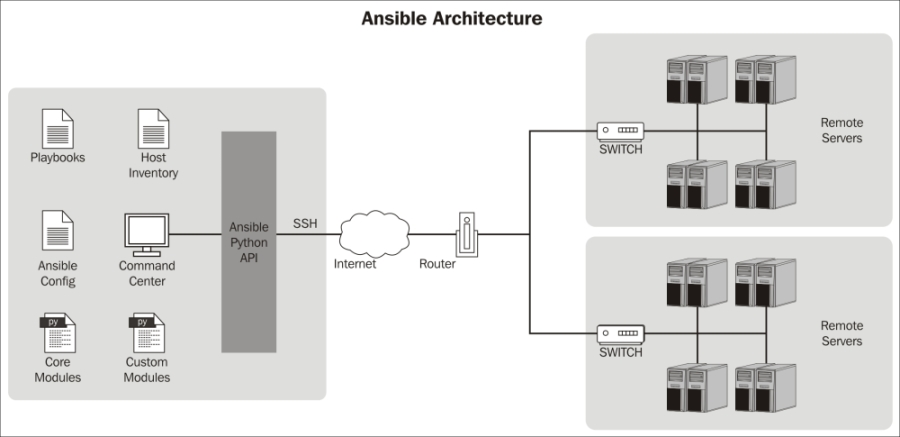
\includegraphics[width=\linewidth]{images/ansible_arch}}
\caption{Ansible Architecture \cite{www-ansible-arch-pic}.}
\label{fig:false-color}
\end{figure}

Like many other configuration management softwares, Ansible
distinguishes two types of servers: controlling machines and
nodes. Ansible uses a single controlling machine where the
orchestration begins. Nodes are managed by a controlling machine over
SSH. The location of the nodes is described by the inventory of the
controlling machine \cite{www-ansible3}.

Modules are deployed by Ansible over SSH. These modules are
temporarily stored in the nodes and communicate with the controlling
machine through a JSON protocol over the standard
output \cite{www-ansible}.

The design goals of Ansible includes consistency, high reliability,
low learning curve, security and to be minimalistic in nature. The
security comes from the fact that Ansible doesn't require users to
deploy agents on nodes and manage remote machines using SSH or
WinRM. If needed, Ansible can connect with LDAP, Kerberos, and other
centralized authentication management systems \cite{www-ansible2}.

\subsection{Advanced Features}

The Ansible Playbook language includes a variety of features which
allow complex automation flow, this includes conditional execution of
tasks, the ability to gather variables and information from the remote
system, ability to spawn asynchronous long running actions, ability to
operate in either a push or pull configuration, it also includes a
check mode to test for pending changes without applying change, and
the ability to tag certain plays and tasks so that only certain parts
of configuration can be applied \cite{www-ansible3}. The features
allow your applications and environments to be modeled simply and
easily, in a logical framework that is easily understood. Ansible has
low overhead and is much smaller when compared to other tools like
Puppet \cite{www-ansible4}.

\subsection{Playbook and Roles}

Playbook is what Ansible uses to perform automation and
orchestration. They are Ansible's configuration, deployment, and
orchestration language. They can be used to describe policy you need
your remote systems to enforce, or a set of steps in a general IT
process \cite{www-ansible5}.

At a basic level, playbooks can be used to manage configurations and
deployments to remote machines. While at an advanced level, they can
be utilized to sequence multi-tier rollouts which involve rolling
updates, and can also be used to delegate actions to other hosts,
interacting with monitoring servers and load balancers at the same time.

Playbooks consist of series of plays, which are used to define
automation across a set of hosts, known as the 'inventory'. These
'play' generally consists of multiple 'tasks', that can select one,
many, or all of the hosts in the inventory where each task is a call
to an Ansible module - a small piece of code for doing a specific
task. The tasks may be complex, such as spinning up an entire cloud
formation infrastructure in Amazon EC2 or Chameleon. Ansible includes
hundreds of modules which help it perform a vast range of tasks
\cite{www-ansible}.

Similar to many other languages Ansible supports encapsulating
Playbook tasks into reusable units called 'roles'. These roles can be
used to easily apply common configurations in different scenarios,
such as having a common web server configuration role which can be
used in development, test, and production automation. The Ansible
Galaxy community site contains thousands of customizable rules that
can be reused used to build Playbooks.

Playbook can be used to combine multiple tasks to achieve complex
automation \cite{www-ansible5}. Playbook and Ansible can be easily used
in implementing a cluster-wide rolling update that consists of
consulting a configuration/settings repository for information about
the involved servers, configuring the base OS on all machines and
enforcing the desired state. It can also be used in signaling the
monitoring system of an outage window prior to bringing the servers
offline and signaling load balancers to take the application servers
out of a load balanced pool \cite{www-ansible}.

\subsection{Integration Of Cloud And Infrastructure}

Ansible can easily deploy workloads to a variety of public and
on-premise cloud environments. This capability includes cloud
providers such as Amazon Web Services, Microsoft Azure, Rackspace,
Cloudmesh, and Google Compute Engine, and local infrastructure such as
VMware, OpenStack, and CloudStack. This includes not just compute
provisioning, but storage and networks as well and the capability
doesn't end here. As noted, further integrations are easy, and more
are added to each new Ansible release. As Ansible is open source,
anyone can make his/her contributions \cite{www-ansible}.

\section{OpenCV}
OpenCV stands for Open Source Computer Vision Library. It is an
extensively used open source machine learning and computer vision
software library. OpenCV was built with a motive to provide a common
infrastructure for computer vision applications and to accelerate the
use of machine perception in the commercial products. Being an open
source library licensed under BSD-licensed product, OpenCV makes it
easy for anyone to utilize and modify the code \cite{www-opencv}.

The library has a number of optimized algorithms, which includes a
comprehensive set of both classic and advanced computer vision and
machine learning algorithms. The algorithms can be used for a variety
of purposes ranging from face detection, object identification,
classification of human actions to tracking moving objects, extracting
3D models of objects. It has C++, C, Python, Java and MATLAB
interfaces and supports Windows, Linux, Android and Mac OS. OpenCV
leans mostly towards real-time vision applications and takes advantage
of single instruction, multiple data (SIMD) and Streaming SIMD
Extensions instructions when available \cite{www-opencv}.

\section{Face Detection}

Face detection is a specific case of object-class detection. In
object-class detection, the task is to find the locations and sizes of
all objects in an image that belong to a given class. Face-detection
algorithms focus on the detection of frontal human faces. It is
analogous to image detection in which the image of a person is matched
bit by bit. Image matches with the image stored in database. Any
facial feature changes in the database will invalidate the matching
process \cite{fd-using-haar}.

\begin{figure}[htbp]
\centering
\fbox{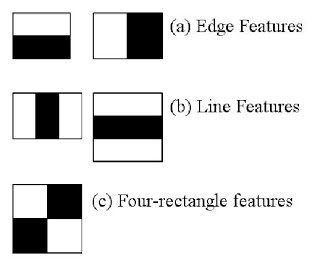
\includegraphics[width=\linewidth]{images/fd_2}}
\caption{Features \cite{fd-using-haar}.}
\label{fig:false-color}
\end{figure}

A number of approaches are used but the most common one which our
project utilized is a method where the possible human eye regions are
detected by testing all the valley regions in the gray-level
image. The basic idea is eyes (white) is separated by darker shades
(skin color) above and below it. Then the genetic algorithm is used to
generate all the possible face regions which include the eyebrows, the
iris, the nostril and the mouth corners \cite{fd-using-haar}.

Each possible face candidates is normalized to reduce lightning effect
caused due to uneven illumination and the shirring effect due to head
movement. The fitness value of each candidate is measured based on its
projection on the eigen-faces. After a number of iterations, all the
face candidates with a high fitness value are selected for further
verification. At this stage, the face symmetry is measured and the
existence of the different facial features is verified for each face
candidate.

We have utilized face detection Haar cascade provided by OpenCV. The
Haar cascade is a classifier achieved using machine learning algorithm
known as AdaBoost \cite{www-adaboost-wiki}. Initially, the AdaBoost
algorithm required a lot of positive images (images of faces) and
negative images (images without faces) to train the face detection
classifier. Then the features are extracted from it. Each feature is a
single value obtained by subtracting sum of pixels under imaginary
white rectangle from sum of pixels under black rectangle
\cite{fd-using-haar}.

\begin{figure}[htbp]
\centering
\fbox{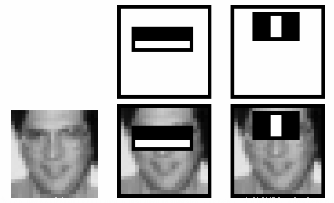
\includegraphics[width=\linewidth]{images/fd_1}}
\caption{Basic idea behind features \cite{fd-using-haar}.}
\label{fig:false-color}
\end{figure}

All possible sizes and locations of each kernel are used to calculate
plenty of features. For each feature calculation, we need to find sum
of pixels under white and black rectangles. Among all the features
generated, most of them are irrelevant. To select best features, they
are applied to each and every feature on all the training images. For
each feature, it finds the best threshold which will classify the
faces to positive and negative. There will be errors or
misclassifications but when results from all the features are combined
the results are excellent. Out of all the features, the features with
the minimum error rate, are the features that best classifies the face
and non-face images.

Final classifier is a weighted sum of these weak
classifiers/features. It is considered as weak classifier because it
can't classify the image alone, but together with other classifiers,
forms a strong classifier. The combined results obtained from all the
features help to identify if a face is present in the image, and if it
is then the classifier also tells the user about the dimensions of the
rectangle and the starting x, y coordinate of that rectange on the
image \cite{www-adaboost-wiki}.

\section{Implementation}
In our implementation, we used Ansible version 2.2.1.0, Mesos version
1.2.0, Python version 2.7.12 and OpenCV version 3.2. The deployment
was done on chameleon cloud.  Firstly, cloudmesh client is set up on
the local machine and ansible is installed. A new security is created
and the ports 5050 and 5051 are exposed. The default security group
was also included which exposed ports 22, 80 and 443. Port 22 is used
for accessing the remote machine. The virtual hardware
template(flavor) used is m1.medium and the image used was
CC-Ubuntu16.04-20161214. A virtual hardware template defines the size
of RAM, disk size, and number of cores. The flavor m1.medium specifies
2 VCPU's used, 40 GB root disk, 4096 MB RAM. The cluster was setup to
have 3 virtual machines(nodes). Amongst the 3 virtual machines, one was
used as Mesos master and the remaining two were used as Mesos
agents(slaves).  The profile details for cloudmesh client have been set
up. The cloudmesh client setup was validated. The system has been
deployed using Ansible roles. For the deployment, the system has been
divided into multiple roles such as inventory role(r\_inventory) ,
role for create swap file(r\_swap), mesos(r\_mesos) role,
master(r\_master) role, agent(r\_agent) role, role for copying
framework(r\_copy\_framework) and role for running
framework(r\_run\_framework).

\section{Roles}
The functionality of the Ansible roles are explained as below:

\subsection{Inventory}
The role r\_inventory was used for inventory setup on the local
machine.  Firstly, the operating cluster was selected and its node
details were obtained. These nodes were added to the known hosts file
under the ssh directory. The inventory was created selecting two nodes
as Mesos agents and one as Mesos master and were tagged accordingly in
the inventory file.

\subsection{Create Swap file}
Swap space in Linux is used when the amount of physical memory is
full. If the system needs more memory resources and the RAM is full,
inactive pages in memory are moved to the swap space. Initially, the
built was unsuccessful when attempts were made with RAM size of 2GB,
4GB and 8GB. It was observed, the virtual machines created had no swap
space defined. The swap size was increased to 2GB after which Mesos
was successfully installed. All these observations led to the
conclusion that for successfully installing Mesos on a virtual machine
minimum of 2GB swap space is required. The playbook r\_create\_swap
successfully creates a swap file of 5GB on all the remote machines.

\subsection{Mesos}
The Mesos package is downloaded from the Mesos website. The latest
version of Apache Mesos is 1.2.0 and it is uncompressed on the virtual
machines. All the existing softwares on the virtual machines are
updated.  The dependencies required for Mesos 16.04 are openjdk-8-jdk,
python-dev, build-essential, python-virtualenv, libcurl4-nss-dev,
libsasl2-dev, libsasl2-modules, maven, libapr1-dev, libsvn-dev,
zlib1g-dev, git. These packages are specific to different distribution
and versions of OSes. Now, the dependencies required for face
detection framework are installed.  The dependencies include
python-pip, numpy and opencv-python to support face detection
framework. In Mesos, applications are deployed as frameworks. Mesos is
configured using the configure command. In order to install Mesos on
the virtual machines, the make and make check commands are executed.

\subsection{Mesos Master}
The Mesos master is run on the host which was selected as the Mesos
master in the inventory file. The working directory for Mesos is
selected. The IP address of this virtual machine is advertised using
the tag --advertise\_ip. The Mesos master runs on default port
5050. The Mesos master can be validated by entering the IP address
followed by the port number of the Mesos master in a Web browser on a
local machine.

\subsection{Mesos Agent}
The Mesos agent is run on the hosts which were selected as the Mesos
agents in the inventory file. The working directory for Mesos is
selected.  The IP address of the Mesos agents are advertised and the
IP address of the master to which the agents will be connected is
specified. In the inventory role, the IP address of the master node
was saved in a separate file which is copied to the remote agents in
this role and the IP address of the master will be used by the agents
to connect to the master node. The agent runs on the default port
5051.

\subsection{Copy and Run framework}
The face detection framework files are copied from the local machine
to all the remote virtual machines including both the Mesos master
node and Master agent nodes and are placed in their respective
directories. The face detection framework is then run on the master node.

\section{Framework Implementation}

\begin{table*}[t]
\centering
\caption{Benchmarks} 
\label{Performance comparison}
\begin{tabular}{|c|c|c|c|c|c|c|c|}
  \hline
  Operating & Flavor & Virtual & RAM & Swap & HDD & Time to & Time to run\\
  System &  & Size & CPU Cores & Size & Size & run make & make install\\
   &  & Allocated & (in GB) & (in GB) & (in GB) & (in hh:mm:ss) & (in hh:mm:ss)\\
  \hline
  Ubuntu 14.04 & small & 1 & 2 & 2 & 20 & 00:43:56 & 00:48:07 \\
  \hline
  Ubuntu 14.04 & medium & 2 & 4 & 5 & 40 & 00:35:23 & 00:42:32 \\
  \hline
  Ubuntu 14.04 & large & 2 & 8 & 5 & 80 & 00:33:27 & 00:37:21 \\
  \hline
  Ubuntu 16.04 & small & 1 & 2 & 2 & 20 & 00:40:32 & 00:48:32 \\
  \hline
  Ubuntu 16.04 & medium & 2 & 4 & 2 & 40 & 00:37:56 & 00:46:68 \\
  \hline
  Ubuntu 16.04 & medium & 2 & 4 & 5 & 40 & 00:19:31 & 00:32:16 \\
  \hline
  Ubuntu 16.04 & medium & 2 & 4 & 7 & 40 & 00:21:47 & 00:29:43 \\
  \hline
  Ubuntu 16.04 & large & 2 & 8 & 5 & 80 & 00:20:31 & 00:31:23 \\
  \hline
\end{tabular}
\end{table*}
The test framework provided by mesos have been modified to run face
detection application. The framework initializes all the requirements
through face\_detection\_framework file after which
face\_detection\_executor runs. The executor creates threads which
then run on agents. The executor is designed such that it can be
easily modified to support another python application by just changing
the call to the main function in run\_task.

The variable dataset and database\_url are the only variables that
need to be modified to change the dataset from which the images need
to extracted and head counts need to be taken. Here, the dataset
variable tells the dataset name and the dataset\_url tells the location
from where the zip folder can be downloaded. The program downloads and
unzips the folder to home directory of the user and this default path can
be changed by changing the global\_path variable. After unzipping the
files, the program removes the zip folder as it is no longer required.

Once the dataset is extracted, the file list is given to the face
detection program implemented using OpenCV library. The OpenCV library
uses cascade files, where the cascade files are simply classifiers
which can identify faces in an image or dogs in an image or any other
object depending on the cascade file used. For our application, face
detection cascade has been used and the link to cascade file is given
in cascase\_url.  One can easily change this cascade file and change
the way this program functions, i.e. one can just provide the
hyperlink in the variable cascade\_url depending on the cascade file
user wants to use and the function will identify dogs, cats, eyes or
any other object which the cascade file is trained to identify. The user
can find these cascade files online, easily or could train and create
one if required.

The program identifies faces, marks them in a rectangle and saves the
output in the output folder. The number of images has been restricted
to 50 for testing purposes but this can easily be changed by updating
the no\_files and images\_per\_file variable as per the
requirement. After the results have been obtained the dataset folder
is deleted. The results obtained contains images with faces marked in
blue square and the count is maintained in results.txt file. These
results are saved on the agent machines which is then copied to
local machine using fetch command automatically.

Whenever new tests are run, the results are appended to results.txt
file in place of just replacing the results. This has been done as a
user might decide to run the application for different dataset or for
different images while keeping the head counts for older datasets.

\section{Benchmark}
The benchmarks are shown in Table 1 which compare the
time to run the make command and the make check on different VMs. The time
required to install, setup a cluster and install prerequisites has been
excluded as they are negligible and on average take 5 minutes on each
VM and just vary in few seconds on average.

\begin{figure}[htbp]
\centering
\fbox{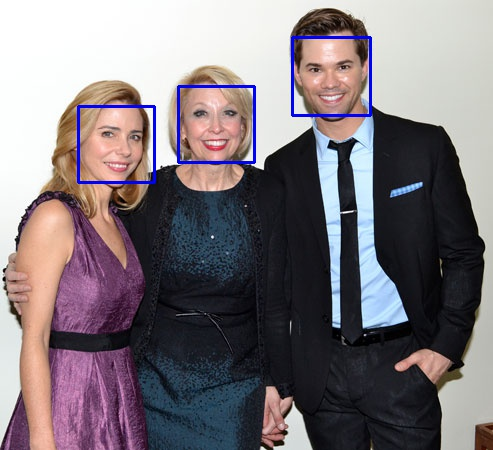
\includegraphics[width=\linewidth]{images/result_img}}
\caption{Sample Output Image.}
\label{fig:false-color}
\end{figure}

\begin{figure}[htbp]
\centering
\fbox{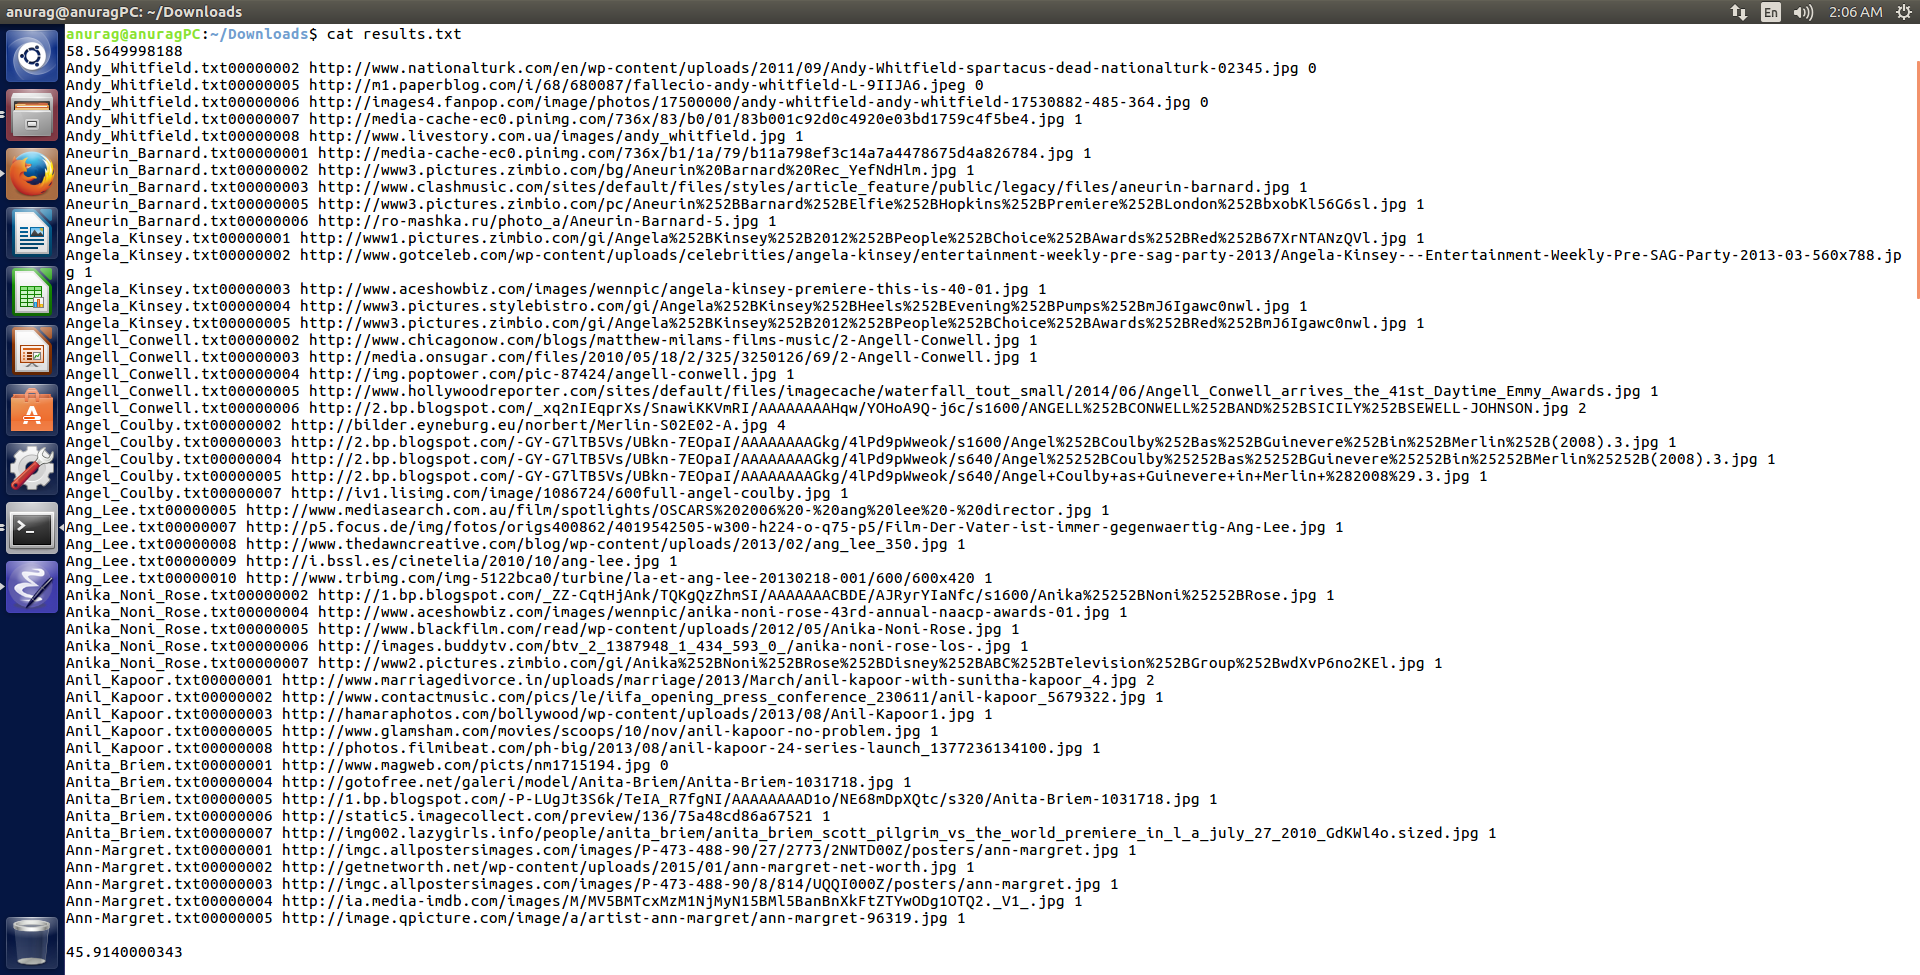
\includegraphics[width=\linewidth]{images/result_txt}}
\caption{Sample Result.}
\label{fig:false-color}
\end{figure}

The results shown in table 2 were run on VM's running Ubuntu 16.04
with flavor as medium and swap size of 5 GB. The results were taken
for 1 image to see how much time initialization takes. The results
show that there is significant improvement when number of agents gets
increased.

\begin{table}[htbp]
\centering
\caption{Application Benchmarks} 
\label{Application Benchmarks}
\begin{tabular}{|c|c|c|}
  \hline
  Number & Run Time & Run Time\\
  Of Images & with 1 Agent & with 2 Agents\\
   & (in hh:mm:ss) & (in hh:mm:ss)\\
  \hline
  1 & 00:00:28 & 00:00:45 \\
  \hline
  50 & 00:01:21 & 00:01:15 \\
  \hline
  100 & 00:02:12 & 00:01:52 \\
  \hline
  500 & 00:05:08 & 00:03:25 \\
  \hline
  1000 & 00:10:21 & 00:07:32 \\
  \hline 
\end{tabular}
\end{table}


\section{Conclusion}
The head count detection framework is running successfully on Apache
Mesos and the output is generated on the local machine which gives the
source of the image and the number of head counts detected in the
image along with it. Apache Mesos was successfully deployed on Linux
16.04 and 14.04 systems and the time required to install and deploy
Mesos was successfully benchmarked. Implementation of the head count
detection framework was successfully tested on Apache Mesos with a
cluster of 1 master with 1 agent and 1 master with 2 agents. Ansible
was used to successfully deploy Mesos on chameleon cloud and it is
seen that Apache Mesos handles the containerization of the framework
with ease. The future scope would include deployment of the headcount
detection framework over 1,000 virtual machines and test the
scalability of Apache Mesos. Along with scalability, the reliability
can also be tested by running multiple masters and checking the fault
tolerance of Apache Mesos.

% Bibliography

\bibliography{references}


\section*{Author Biographies}
	\begingroup \setlength\intextsep{0pt}
	\begin{minipage}[t][3.2cm][t]{1.0\columnwidth}
	% Adjust height [3.2cm] as required for separation of bio photos.
	  \begin{wrapfigure}{L}{0.25\columnwidth}
	    
\includegraphics[width=0.25\columnwidth]{images/john_smith.eps}
	  \end{wrapfigure}
	  \noindent
	  {\bfseries Anurag Kumar Jain} will receive his Masters (Computer Science)
	  in 2018 from The Indiana Univeristy Bloomington. His research
	  interests include Artificial Intelligence and Big Data.
	\end{minipage}
	\begin{minipage}[t][3.2cm][t]{1.0\columnwidth} % Adjust height [3.2cm] as required for separation of bio photos.
	  \begin{wrapfigure}{L}{0.25\columnwidth}
	    
\includegraphics[width=0.25\columnwidth]{images/alice_smith.eps}
	  \end{wrapfigure}
	  \noindent
	  {\bfseries Pratik Sushil Jain} will receive his Masters (Computer
	  Science) in 2018 from Indiana University Bloomington. His research
	  interests include Big Data and Machine Learning.
	\end{minipage}
	\begin{minipage}[t][3.2cm][t]{1.0\columnwidth} % Adjust height [3.2cm] as required for separation of bio photos.
	  \begin{wrapfigure}{L}{0.25\columnwidth}
	    
\includegraphics[width=0.25\columnwidth]{images/alice_smith.eps}
	  \end{wrapfigure}
	  \noindent
	  {\bfseries Ronak Parekh} will receive his Masters (Computer
          Science) in 2018 from Indiana University Bloomington. His
          research interests include Big Data, Cloud Computing and
          Machine Learning.
	\end{minipage}
        \endgroup
        
\end{document}
